%%%%%%%%%%%%%%%%%%%%%%%%%%%%%%%%%%%%%%%%%%%%%%%%%%%%%%%%%%%%%%%%%%%%%%%%%
%                                                                       %
%              A template file for usage with ustthesis.cls             %
%                                                                       %
%%%%%%%%%%%%%%%%%%%%%%%%%%%%%%%%%%%%%%%%%%%%%%%%%%%%%%%%%%%%%%%%%%%%%%%%%

\documentclass{ustthesis}
\usepackage{nicematrix,booktabs}
\usepackage{threeparttable}
\usepackage{amsmath, amssymb, amsfonts, bm}
\usepackage{algorithm}
\usepackage{algorithmic}
\usepackage{color,graphicx}
\usepackage{siunitx}
\usepackage{soul}
\usepackage{graphics} % for pdf, bitmapped graphics files
\usepackage{subcaption}
\usepackage[round]{natbib}
\newtheorem{proof}{Proof}
\usepackage{bookmark}
\usepackage{hyperref} % for better viewing experience  -- added by alan
\usepackage{textcomp}
\usepackage{multirow}
\usepackage{nth}
\usepackage{indentfirst}
\usepackage{siunitx}
\usepackage{changepage}
\usepackage[a4paper, margin=25mm,textheight=247mm,textwidth=145mm]{geometry} % page requriement from the university ---added by Lei.
\usepackage{fancyhdr}
\usepackage[inline]{enumitem}
\newlist{myenumerate}{enumerate*}{1}
\setlist[myenumerate]{itemjoin=\\,label=\arabic*),after=\\}
% Alan: begin the font trial
% Euler for math | Palatino for rm | Helvetica for ss | Courier for tt
% \renewcommand{\rmdefault}{ppl} % rm

% NOTE Lei: rouphly 32 lines for 12pt font size and 1.5 line spacing
\linespread{1.05}

% \usepackage[scaled]{helvet} % ss
% \usepackage{courier} % tt
% \usepackage{euler} % math
% \usepackage{eulervm} % a better implementation of the euler package (not in gwTeX)
% \normalfont
% \usepackage[T1]{fontenc}
% Alan: end the font trial


\DeclareMathOperator*{\argmax}{\arg\!\max}
\DeclareMathOperator*{\argmin}{\arg\!\min}

\newcommand{\red}[1]{#1}
\newcommand{\tab}[1]{\hspace{3mm}}

% NOTE Lei: personal habit for math symbols.
\newcommand{\bx}{\mathbf{x}}
\newcommand{\bX}{\mathbf{X}}
\newcommand{\by}{\mathbf{y}}
\newcommand{\bY}{\mathbf{Y}}
\newcommand{\bD}{\mathbf{D}}
\newcommand{\bE}{\mathbf{E}}
\newcommand{\ba}{\mathbf{a}}
\newcommand{\bs}{\mathbf{s}}
\newcommand{\bn}{\mathbf{n}}
\newcommand{\bI}{\mathbf{I}}
\newcommand{\bsigma}{\mathbf{\sigma}}
\newcommand{\cS}{\mathcal{S}}
\newcommand{\cX}{\mathcal{X}}
\newcommand{\cA}{\mathcal{A}}
\newcommand{\cB}{\mathcal{B}}
\newcommand{\cD}{\mathcal{D}}
\newcommand{\bu}{\mathbf{u}}
\newcommand{\bv}{\mathbf{v}}
\newcommand{\ts}{\textsuperscript}
\newcommand{\etal}{{\em et al.}}
\newcommand{\norm}[1]{\left\lVert#1\right\rVert}
\DeclareMathOperator{\atantwo}{atan2}
\newcommand{\argminE}{\mathop{\mathrm{argmin}}}
\numberwithin{equation}{section}

\setcounter{tocdepth}{3}
\setcounter{secnumdepth}{3}


% \renewcommand{\familydefault}{\rmdefault}

% \usepackage{latexsym}
    % Use the "latexsym" package when encountering the following error:
    %   ! LaTeX Error: Command \??? not provided in base LaTeX2e.
% \usepackage{epsf}
    % Use the "epsf" package for including EPS files.

%%%%%%%%%%%%%%%%%%%%%%%%%%%%%%%%%%%%%%%%%%%%%%%%%%%%%%%%%%%%%%%%%%%%%%%%%
%                                                                       %
% Preambles. DO NOT ERASE THEM. Change to suite your particular purpose.%
%                                                                       %
%%%%%%%%%%%%%%%%%%%%%%%%%%%%%%%%%%%%%%%%%%%%%%%%%%%%%%%%%%%%%%%%%%%%%%%%%

\title{Forecasting the Ammonia Concentration and Color Level in Reclaimed Water using Machine Learning}  % Title of the thesis.
\author{Ting~Hsi~LEE}     % Author of the thesis.

% NOTE Lei: choose your degree
\degree{\MPhil}             % Degree for which the thesis is.
% %% or
% \degree{\PhD}              % Degree for which the thesis is.

\department{Civil~and~Environmental~Engineering}       % Department to which the thesis

\advisor{Prof.~Chii~SHANG}     % Supervisor.

% NOTE Lei: Uncomment this line if you have a co-supervisor/co-advisor
% \coadvisor{Prof.~Mazi~Zhang}     % Co Supervisor.

\depthead{Prof.~Meimei~Han}    % department head.

\defencedate{2022}{08}{08}      % \defencedate{year}{month}{day}   NOTE Lei: change it to the submission month when you submit your final version.

% NOTE:
%   According to the sample shown in the guidelines, page number is
%   placed below the bottom margin.  However, if the author prefers
%   the page number to be printed above the bottom margin, please
%   activate the following command.
% \PNumberAboveBottomMargin

\graphicspath{{./figure/}}
\begin{document}

%%%%%%%%%%%%%%%%%%%%%%%%%%%%%%%%%%%%%%%%%%%%%%%%%%%%%%%%%%%%%%%%%%%%%%%%%
%                                                                       %
% Now the actual Thesis. The order of output MUST be followed:          %
%                                                                       %
%    1) TITLEPAGE                                                       %
%                                                                       %
% The \maketitle command generates the Title page as well as the        %
% Signature page.                                                       %
%                                                                       %
%%%%%%%%%%%%%%%%%%%%%%%%%%%%%%%%%%%%%%%%%%%%%%%%%%%%%%%%%%%%%%%%%%%%%%%%%
\maketitle

%%%%%%%%%%%%%%%%%%%%%%%%%%%%%%%%%%%%%%%%%%%%%%%%%%%%%%%%%%%%%%%%%%%%%%%%%
%                                                                       %
%     2) DEDICATION (Optional)                                          %
%                                                                       %
% The \dedication and \enddedication commands are optional. If          %
% specified it generates a page for dedication.                         %
%
%%%%%%%%%%%%%%%%%%%%%%%%%%%%%%%%%%%%%%%%%%%%%%%%%%%%%%%%%%%%%%%%%%%%%%%%%

% \dedication
% This is an optional section.
% \enddedication

%%%%%%%%%%%%%%%%%%%%%%%%%%%%%%%%%%%%%%%%%%%%%%%%%%%%%%%%%%%%%%%%%%%%%%%%%
%                                                                       %
%     3) SIGNATURE                                                      %
%                                                                       %
% \signature and \endsignature defines the                              %
% signature page of the Thesis especially for ece.                      %
%                                                                       %
%%%%%%%%%%%%%%%%%%%%%%%%%%%%%%%%%%%%%%%%%%%%%%%%%%%%%%%%%%%%%%%%%%%%%%%%%
%%Remove when convertring to work
\signature
		\begin{figure}[!hb]
		\begin{tabular}{ll}

    %% NOTE Lei:
    %%   In case the space is not enough, try \footnotesize for this part.
		% \footnotesize{Thesis Examination Committee} &  \\[8pt]
		% \footnotesize{1. Prof. xxx (Supervisor)}   &  \footnotesize{Department of Electronic and Computer Engineering} \\[8pt]
		% \footnotesize{2. Prof. xxx}   &  \footnotesize{Department of Electronic and Computer Engineering} \\[8pt]
		% \footnotesize{3. Prof. xxx}   &  \footnotesize{Department of Electronic and Computer Engineering} \\[8pt]
		% \footnotesize{4. Prof. xxx}            &  \footnotesize{Department of Mathematics }\\[8pt]
		% \footnotesize{5. Prof. xxx (External Examiner)}  & \footnotesize{Department of Electrical Engineering and} \\[8pt]
		%                               & \footnotesize{Information Technology} \\[8pt]
		%                               &  \footnotesize{Vienna University of Technology} \\[8pt]
    %% NOTE Lei:
    %%  PhD thesis does not need to record the chairperson here. If you have a co-supervisor, please add the Co-supervisor line manually.
		\end{tabular}
		\end{figure}
\endsignature

%%%%%%%%%%%%%%%%%%%%%%%%%%%%%%%%%%%%%%%%%%%%%%%%%%%%%%%%%%%%%%%%%%%%%%%%%
%                                                                       %
%     3) ACKNOWLEDGMENTS                                                %
%                                                                       %
% \acknowledgments and \endacknowledgments defines the                  %
% Acknowledgments of the author of the Thesis.                          %
%                                                                       %
%%%%%%%%%%%%%%%%%%%%%%%%%%%%%%%%%%%%%%%%%%%%%%%%%%%%%%%%%%%%%%%%%%%%%%%%%
%%Remove when convertring to work
\acknowledgments

I would first express my enormous gratitude to my thesis supervisor Prof. Chii Shang for giving me the opportunity to start my MPhil degress in this research group. I was given chances to expose to different research topics and work with other students, most important, I have learned so much from his mentoring.  He also encourage me to develop the research area I am interested in. I was benefited from his knowledge in this domain and his wisdom in 


I would first express my gratitude to my supervisor Prof. Chii SHANG for giving me patient instruction and continuous support during my MPhil study. He encouraged me to learn from mistakes and move forward in steady steps with new-found wisdom. I benefited a lot from his explicit guidance on critical thinking during research and teaching. He has been an excellent mentor and I sincerely appreciate the opportunity to work with him.

I really appreciate Prof. Guanghao CHEN and Prof. Bo SUN for serving on my thesis examination committee. Special thanks should go to Mr. Ran YIN and Miss. Yingying XIANG for giving critical and constructive suggestions on my research.

Thanks also go to technical staff including Mr. Shing Tak LUI, Mr. Wai Lun Johnson YAU and Mr. Chi Man HO for their assistance in instrumentation operation and maintenance.

With great pleasure, I would like to thank my groupmates, labmates and friends for their assistance and friendship.

Finally, I would like to express my gratitude to my family for their love, support and continuous encouragements.

\endacknowledgments


%\clearpage
%\phantom{s}
%\thispagestyle{empty}
%%%%%%%%%%%%%%%%%%%%%%%%%%%%%%%%%%%%%%%%%%%%%%%%%%%%%%%%%%%%%%%%%%%%%%%%%
%                                                                       %
%     4) TABLE OF CONTENTS                                              %
%                                                                       %
%%%%%%%%%%%%%%%%%%%%%%%%%%%%%%%%%%%%%%%%%%%%%%%%%%%%%%%%%%%%%%%%%%%%%%%%%

\tableofcontents

%%%%%%%%%%%%%%%%%%%%%%%%%%%%%%%%%%%%%%%%%%%%%%%%%%%%%%%%%%%%%%%%%%%%%%%%%
%                                                                       %
%     5) LIST OF FIGURES (If Any)                                       %
%                                                                       %
%%%%%%%%%%%%%%%%%%%%%%%%%%%%%%%%%%%%%%%%%%%%%%%%%%%%%%%%%%%%%%%%%%%%%%%%%

\listoffigures

%%%%%%%%%%%%%%%%%%%%%%%%%%%%%%%%%%%%%%%%%%%%%%%%%%%%%%%%%%%%%%%%%%%%%%%%%
%                                                                       %
%     6) LIST OF TABLES (If Any)
%                                                                       %
%%%%%%%%%%%%%%%%%%%%%%%%%%%%%%%%%%%%%%%%%%%%%%%%%%%%%%%%%%%%%%%%%%%%%%%%%

\listoftables

%%%%%%%%%%%%%%%%%%%%%%%%%%%%%%%%%%%%%%%%%%%%%%%%%%%%%%%%%%%%%%%%%%%%%%%%%
%                                                                       %
%     7) ABSTRACT                                                       %
%                                                                       %
% \abstract and \endabstract are used to define a short Abstract for    %
% the Thesis.                                                           %
%                                                                       %
%%%%%%%%%%%%%%%%%%%%%%%%%%%%%%%%%%%%%%%%%%%%%%%%%%%%%%%%%%%%%%%%%%%%%%%%%

\begin{abstract}

Water scarcity is a global challenge. One of the promising ways to mitigate the 
water resource crisis is via wastewater reclamation. Chlorine is commonly used 
for reclaimed water disinfection and requires precise dosing to satisfy endorsed 
quality standards. Ammoniacal nitrogen (NH$_{3}$N) and colour exist in the reclaimed 
water at concentrations between 0.23 – 5.44 mg N/L and 80 – 150 Hazen units, 
respectively, and can affect the chlorine demand. Forecasting the reclaimed water 
quality enables a feedback control system over the disinfection process by predicting 
the exact chlorine dose required which secures sufficient time to respond to sudden 
surges in color and ammonia levels. This study developed time-variant models based on 
machine learning to predict the NH$_{3}$N concentration and colour three hours into the 
future in the reclaimed water. The NH$_{3}$N data was collected by an online analyzer, and 
colour data was collected by a customized auto-sampling spectrophotometer, both are 
installed in the reclaimed water treatment plant in Hong Kong. Long Short-Term Memory 
(LSTM) was found to be the most effective architecture for training NH$_{3}$N and colour 
forecasting models. In the training processes, we applied data pre-processing methods 
and feature engineering, a technique to select or create relevant variables in raw data 
to enhance predictive model performance. From feature engineering, we discovered that the 
daily fluctuation in NH$_{3}$N and colour has correlations with the urban water consumption patterns. 
This finding further enhanced the NH$_{3}$N and colour forecasting model performance by 4.9\% 
and 5.4\% compared to baseline models. This research work offers novel methods and feature 
engineering processes for NH$_{3}$N concentration and colour forecasting in reclaimed water 
for treatment optimization. 

\end{abstract}


%%%%%%%%%%%%%%%%%%%%%%%%%%%%%%%%%%%%%%%%%%%%%%%%%%%%%%%%%%%%%%%%%%%%%%%%%
%                                                                       %
%     8) The Actual Contents                                            %
%                                                                       %
% The command \chapters MUST BE USED to ensure that the entire content  %
% of the Thesis is double-spaced (in version 1.0).                      %
%                                                                       %
% However, in version 2.0, \chapters will be automatically added in     %
% the beginning of the first chapter.                                   %
%                                                                       %
%%%%%%%%%%%%%%%%%%%%%%%%%%%%%%%%%%%%%%%%%%%%%%%%%%%%%%%%%%%%%%%%%%%%%%%%%

%%\chapters         % Not necessary with ustthesis.cls (v2.0).

%%%%%%%%%%%%%%%%%%%%%%%%%%%%%%%%%%%%%%%%%%%%%%%%%%%%%%%%%%%%%%%%%%%%%%%%%
%                                                                       %
% Each chapter is defined via the \chapter command. The usual sectional %
% commands of LaTeX are also available.                                 %
%                                                                       %
%%%%%%%%%%%%%%%%%%%%%%%%%%%%%%%%%%%%%%%%%%%%%%%%%%%%%%%%%%%%%%%%%%%%%%%%%


\chapter{Introduction}

\section{Background}

%paragraph 1 Forecasting models play an important role in water quality control in DTPs and WWTPs.
%paragraph 2 Water reclamation-why is it a good choice for solving urban water scarcity
%paragraph 3 Decision-making processing-how does this help water reclamation
%paragraph 4 Deep learning model to replace fuzzy supervisor and machine learning models-the need of using it
AI technologies have been successfully applied to different DWT processes, such as the prediction of the coagulant 
dosage, discrimination of the DBP formation potential, advanced control of membrane fouling, membrane preparation 
and optimization, and water quality prediction. \cite{liRecentAdvancesArtificial2021}

%%%% Paragraph 1
Forecasting models play an important roles in water quality control in drinking water treatment plants (DTPs) 
and wastewater treatment plants (WWTPs). The need of using forecasting models are becuase the unpredictable 
nature of water quality, and the treatment operations are subjected to the change of water quality to prodcue
effluent complied the government regulation \cite{chenAssessingWastewaterReclamation2003}

%%%% Paragraph 2
Forecasting models can also be called time series model becuase the data is consisted of the values and the 
time (need to be further revised). For the well-know time series models are for example, RNN, ... These are 
used to replace the theory-based models, for example Activated Sludege Model (ASM). The difference between 
these two models are, machine learning based models require to learn from historic data, while the thoery-based
models only need to enter the basic operational parameters (e.g., influent flow, tempearture, and pH, etc).

%%%% Paragraph 3
Despite the promising usage and performance of machine learning models, the collection of the data became
the most difficult tasks. Many small scale or old treatment plants do not have the capital or the available
environment for the set-ups of the online sensors to collect data.
Although these are the major issues, it's still possible to train a forecasting model with one input, which 
is also called a self-prediction model. Although the accuracy or stability compared to multi-input models, 
the forecasted results can be used at some cases. To increase the model performance, there are several ways.
Paper included weather data, or perform data-preprocessing methods to improve the model performance.

%%%% Paragraph 4
These solutions (data preprocessing, feature engineering) are not well discussed in this field, also the 
potential of using univariate models are under estimated.

Keeping an effective disinfectant residual concentration in reclaimed water is still a challenge, due to its high levels of ammonia and organic matter when compared with those in drinking water. \citep{costaIdentificationModellingChlorine2021}


%\begin{figure}[!t]
%   \centering
%   \includegraphics[width=0.75\columnwidth]{imgs/fix-length-time-window.png}
%   \caption{The network structure for the actor-evaluation estimation. It is a combination of convolutional networks for feature extraction and fullyconnected layers for policy learning. They have been separately proven to be effective in our previous works.}
%   \label{fig:ob_network_structure}
%\end{figure}

\section{Objectives}
\noindent
The specific objectives of this thesis work are:\\
%should be investigate the effluent water quality in SWHEPP?
(1) To build baseline univariate forecasting models using machine learning and deep learning models.\\
(2) To develop data preprocessing methods for enhancing model forecasting performance.\\
(3) To extract features and hidden relations of water parameters in MBR effluent by analyzing the wastewater collected upstream of the WWTPs.\\
(4) To develop methods for improving performance of forecasting models using the hidden features and relations of the water parameters.

\section{Organization of the thesis}
In Chapter 1, “Introduction”, the background information, objectives and organization of the thesis were presented.

Chapter 2, “Literature Review”, provides the overview of water quality process controls, the reviews cover the water treatment plant, wastewater treatment plant, and in reclaimed water system.
....

In Chapter 3, “Materials and Methods”, the instruments for ammonia and colour data collection, programming environment, and data preparation methods were summarized. The processes of the formulation of extra features for training forecasting models were illustrated.

In Chapter 4, “Results and discussion”, the performance of machine learning and deep learning models were compared. Forecasting models trained by different data pre-processing methods and the effect of feature engineering were both compared with the baseline model performance. 

In Chapter 5, “Conclusions and Recommendations”, the findings obtained from this thesis work were summarized and the possible future studies were recommended.
\chapter{Literature Review}
%\label{sec:ob_rel}
\section{Introduction to water quality control}
\subsection{Automated system for water quality control}
%%%%%%%%%%PLC and some real application cases in WTP
%Explain PLC better by \cite{WasteWaterTreatment2018}
%re organize this section
Programmable logic controller (PLC) is an industrial computer system designed for any process requiring a series of devices and equipment operates cohesively to achieve multiple purposes in manufacturing or treatment processes. The main components of PLC include a center process unit (CPU), input modules and output modules (I/O). CPU is responsible to process digital signals from input modules and send commands through output modules based on the control logics programmed on the PLC. For chemical dosing control in water treatment plants (WTPs), PLC system receives readings from turbidity and pH sensors and uses pumps to dose aluminum solution automatically \citep{andhareSCADAToolIncrease2014}. The PLC system with the capability of producing real-time output commands in response to the input sigals also makes it widely used in the wastewater treatment plants (WWTPs). For oxygen concentration control in the aeration tank, PLC system receives signals of dissovled oxygen (DO) detectors and transmits signals to open or close the electric butterfly valves to further alter the DO concentration \citep{zhuApplicationPLCSewage2017}. Although PLC systems are the most used system across industries for its easy programming and reliable control, PLC system is merely a device that can be programmed to control operative devices with on-off logic (i.e., a logic control with two states) and the capability of complex control is compromised. In reality, many WTPs or WWTPs have the need of precise control of the treatment processes. Being awared of the limitations of the PLC systems, a more advanced controller called proportional–interal–derivative (PID) controller for receiving analog signals was developed to obtain more sophisticated controls over the operative devices.

%%%%%%%%%%PID and examples
%PID control is used where greater levels of precision in control are required. It combines three control terms to give a single output to drive the setpoint. 
To react to rapidly-changing process conditions, a PID controller generates an output value based on continuous calculation of an error value e(t) as the difference between a desired setpoint (SP) and a measured process variable and applies a correction based on proportional, integral, and derivative terms. The use of the "P", "I", and "D" allows the system to quickly reach steady state with a feedback control system (i.e., the system output is returned to the system input which is included in the decision making process in PID controller). Generally speaking, a PID controller is a technology (i.e., a specialist algorithm) for contorlling a single device with more complex logics, while a PLC system is a physical system consists of different modules and capable of controlling dozens of devices only with two-state logic. In addition, A PID controller can be designed to operate on PLC device and provide a more precise control strategy to a designated device. In WWTPs, a single-variable feedback analog control loop in PID can be used to control the temperature in the activated sludge treatment by stablizing the system temperature in a shorter time \citep{badosDesignPIDControl2020}. The feedback control scheme is also applied in WTPs to adjust the addition of chlorine dosage (i.e., also known as the disinfection process, chlorination, or postchlorination) to reach the target concentration of free chlorine residual (FRC) \citep{wangCompositeControlPostChlorine2019}. Disinfection process is carried out in a chlorine contact tank which provides sufficient time for chlorine to disinfect pollutants. Since the chlorine added by the dosing device requires time to travel from the entry to the exit, the system output can only reflect the changes of water quality in a delayed time of 30 minutes (i.e., the designed time for water to travel in chlorine contact tank is usually 30 minutes or longer). In the case of chlorination, the lag of time makes feedback control difficult \citep{kobylinskiLineControlStrategies2006} as the system is delayed in responding to any sudden surge of the pollutants when it can only receive output at the end of the disinfection process. PID controllers in WWTPs also encounter similar challenges as the increasing complexity of water quality and stricter regulations on the discharged water quality. 

%%%%%%%%%%Transition to how the algorithms in PID can be replace by AI, ML, 
%Introduce to MPC, feedforward control in comparison with PID controller
%The use of mathematical modeling is not ideal, turning to the use of AI modeling
To tackle the difficulties encountered in process control system, many control strategies are proposed, such as feed forward-feedback control, linearized and optimal control, model-predictive control, and fuzzy control, etc \citep{demirFeedbackControlChlorine2014a}. Among the algorithms used in control strategies, Artificial Intelligence (AI) modeling has gained the most attentions in recent years compared to modeling based on mathematical models or empirical formulas. In WTPs or WWTPs, to fully understand the physical, biological, and chemical interactions in the treatment plants is very difficult. The unpredictable behaviors during the water treatment can be the significant changes of influent flow rate, flucutations of water quality, the complexity of biological treatment process, and the large time delay exists between this control variable and the process input, etc. Therefore, AI modeling shows a great potential in dealing with the highly complex conditions in the treatment process \citep{liRecentAdvancesArtificial2021}. In the next sections, the applications of different AI modeling methods will be discussed.

\subsection{Artificial Intelligence}
%AI include fuzzy logic, a subset of ML. ML includes SVM, a subset of DL. DL includes LSTM.
Artificial intelligence (AI) can perform cognitive tasks with the development of computational solutions. The concepts of AI are usually confused, in fact, AI is a very broad term and any kind of algorithms or models which involved in decision-making with computation fall in the domain of AI. For example, fuzzy logic and optimization algorithm are formulated with human design and computer decision making process. There are another subset of AI called machine learning (ML), but the process of generating a ML model is different to generating a fuzzy logic model. ML uses learning algorithms to generate a model via learning from historical or large amount of data without being explicitly programmed. ML algorithms can be classified into three categories, which are Supervised, Unsupervised, and Reinforcement learning. In the training process of supervised learning, input variable (x) and output variable(Y) we will provided, and model will learn from the provided dataset to map the x to the Y. A trained supervised model can generate a prediction for the response to the new data (i.e., also called the unseen data). Unsupervised learning is when the dataset is not labelled, the model can learn to infer patterns in the dataset without reference to the known outputs. This type of algorithm can find similarities and differences in the data. In reinforcement learning, models are designed to constantly interact with the environment in a try-and-error way and recieved rewards and punishments based on the purpose of the tasks. Generating a optimal action to achieve lowest penalties is the main function of a reinforcement learning model. In process control, supervised learning are frequently used in many senarios.

Regression is a supervised machine learning technique used to predict continuous values. A regression model can estimate the relationship between the input variables in the system and the output target from a given dataset, and then use the nonlinear relationship to map the unseen input data to a predicted output data. This type of application is sutiable for water quality prediction  \citep{librantzArtificialNeuralNetworks2018}, and sensor fault detection \citep{cecconiSoftSensingOnLine2021}, etc. 

Fuzzy logic (FL) control is still an effective strategy for process control, and this type of AI modeling is called reasoning. Fuzzy logic is described as an interpretative system in which objects or elements are related with borders not clearly defined, granting them a relative membership degree and not strict, as is customary in traditional logic. The typical architecture of a fuzzy controller, shown in Figure 3, consists of a fuzzifier, a fuzzy rule base, an inference engine, and a defuzzifier \citet{santinFuzzyControlModel2015} proposed a hybrid control system comprised of FL controller and model predictive control using optimizaion model to control the chlorine dosing in a WTP. FL controller and optimzation model fall in the domain of AI, which is excluded from the subset of ML.

Fuzzy logic (FL), a method based on multi-valued logic, uses fuzzy sets to study fuzzy judgement, which allows FL-based fuzzy inference systems to simulate the human brain to implement natural inference [40].The adaptive fuzzy neural inference system (ANFIS) composed of FL and ANN with an inference mechanism has high interpretability compared to common ANN. The combined model has been used to control coagulant dosing systems [41,42].

\subsection{Machine learning and deep learning}
In machine learning, popular models which are frequently used by the researchers for training predictive models are Supporting Vector Machine (SVM), Random Forest (RF), and Artificial Neural Networks (ANN). \citet{librantzArtificialNeuralNetworks2018} trained a RF model to predict the free residual chlorine concentration (FRC) in a WTP, and \citet{xuAlternativeLaboratoryTesting2021} built a RF-based model to predict total nitrogen concentration in water bodies. \citet{guoPredictionEffluentConcentration2015} compared the reliability and accuracy of an ANN model and a SVM model in predicting 1-day interval T-N concentration in a WWTP, and the results showed that RF model has higher accuracy while ANN model is more reliable for assisting decision-making process.

As the the computing power doubled every 18 months according to Moore's law. A subset of ML, Deep Learning (DL) becomes more accessible for sovling everyday issues. In simplicity, DL models can be defined as neural networks with more than two hidden layers (i.e., the model complexity increased and required more computing power to calculate). In DL, there are various types of architectures designed based on the type of problems. For image processing, Convolutional Neural Network (CNN) is designed to extract important features from the image vectors. Another popular DL architecture is Recurrent Neural Network (RNN), which is powerful in solving time series-related applications and Natural Language Processing (NLP) tasks \citep{liERNNDesignOptimization2018}. Although each architecture has their strengh in tackling different types of problems, both architectures can be used for a single task \citet{liPredictionFlowBased2022} built a regression CNN-RNN model for rainfall-runoff prediction. DL can be extremely powerful when multiple architectures ared fused into a single model to perform a specific task, which cannot be realized by machine leraning models. That being said, DL can achieve higher model performance in terms of the prediction accuracy compared to ML. 

\section{Water quality control with machine learning}
%%it's better to find papers that can provide comparison between DL and ML or traditional models
\subsection{Drinking water treatment plants}
%Background
A drinking water treatment plant (DWTPs) produces potable (i.e., drinking water) water for human consumptions by removing contaminants from the source water, such as lake or stream, or from an underground aquifer. The raw water enters DWTPs and goes through treatmet units of coagulation, flocculation, sedimentation, filtration, and disinfection in sequence as the primary treatment scheme in the conventional DWTPs \citep{liRecentAdvancesArtificial2021}. 

%detailed functions of the treatment process
1.8.1 Drinking Water Treatment Drinking water treatment plant could be classified into: – Disinfection plant which is used for high-quality water source to ensure that water does not contain pathogens – Filtration plant: this is usually used to treat surface water – Softening plant which is used to treat groundwater Typical filtration plant is shown in Fig. 5 which is designed to remove odors, color, and turbidity as well as bacteria and other contaminants. Filtration plant employs the following steps: a.Rapid mixing : where chemicals are added and rapidly dispersed through the water b.Flocculation : Chemicals like alum (aluminum sulfate) are added to the water both to neutralize the particles electrically and to make them come close to each other and form large particles called flocs that could more readily be settled out c.Sedimentation : During sedimentation, floc settles to the bottom of the water supply, due to its weight d.Filtration: Once the floc has settled to the bottom of the water supply, the clear water on top will pass through filters of varying compositions (sand, gravel, and charcoal) and pore sizes in order to remove fine particles that were not settled, such as dust, parasites, bacteria, viruses, and chemicals e.Disinfection : involves the addition of chemicals in order to kill or reduce the number of pathogenic organisms



During the treatment processed, colloids, suspended matter, pathogenic microorganisms and organic matter are removed to meet the regulated standard. However, the quality of raw water isn't always stable, and corresponding actions are required to be promptly adopted when events like the surge of pollutants or the large variability of the influent flow. In any event, the treated water from DWTPs should generate drinking water which complies the World Health Organization's Guidelines (WHO's guideline) for drinking water quality. Otherwise, the treated drinking water should either be discharged and result in the short term outage of water supply to the downstream cities or the users will receive contaminated drinking water which can potentially transmit diseases and cause illness.

%Turbidity
Turbidity is one of the critical water quality indicators, which can be defined as the "optical quality" of water, and the unit to decribe the turbidity is called Nephelometric Turbidity Unit (NTU). High levels of turbidity in raw water can impede the effectiveness of filtration and chlorination processes, and potentially cause short-term outages of water supply. Heavy rainfall and fissures within the aquifer can also lead to turbidity events are mostly likely to cause high turbidity \citep{worldhealthorganizationWaterQualityHealth2017}. The challenge in event of high turbidity in raw water is it occurs rapidly and mitigating activities must be actionable immediately. To address sudden event of such, \citet{stevensonAdvancedTurbidityPrediction2019} trained forecasting models based on general linear model (GLM) and RF to predict the time when the turbidiy reaches higher than 7 NTU. The results indicate both model can successfully predict the events (i.e., with accuracy between 0.81 and 0.86), and RF model is found to have higher precision due to it's ability to capture the nonlinear relationship between rainfall (mm) and turbidity (NTU).

%Coagulation dose
To maintain operational costs and water quality in the coagulation process, the amount of coagulant, which is mainly subject to the turbidity and alkalinity in the raw water, is traditionally determined thourgh manually sampling and analysis. Jar test is designed to find out the optimal chemical dosage for coagulation to remove the turbidity in raw water, and the entire process includes on-site sampling and up to more than 40 minutes of laboratory works \citep{ganiEffectPHAlum2017}. To replace the laborious procedure of jar tests, \citet{wangIntegratingWaterQuality2022} proposed using principal component regression (PCR), support vector regression (SVR), and long short-term memory (LSTM) neural network to build predictive models for outputing daily estimated chemical dosage. Compared with linear PCR model, nonlinear SVR and LSTM models captures more relationship between the chemical dose (e.g., ferric sulfate) and the raw water quality based on a higher R-squared value of 0.70.

%membrane-filtration modeling

%Disinfection
Disinfection is the last step of water treatment processes in drinking water treatment plants to generate safe potable water. In this step, one or more chemical disinfectants like chlorine, chloramine, or chlorine dioxide are added into the water to inactivate any remaining pathogenic microorganisms. However, the chlorination process requires precise dosing of disinfectant---too high will lead to the formation of disinfection byproducts (DBPs), and too low will result in insufficient levels of the residaul disinfectant concentration. In both senarios, the treated drinking water can pose health threats to the end users. The aforementioned PID controller can achieve automatic dosing of disinfection, however, \citet{wangModelPredictiveControl2020} found out that the accuracy of the predicted disinfectant dosage using (i.e., chlorine is used in this paper) a Support Vector Regression (SVR) model outperformed a PID controller in both simulation and experimental conditions. An Artificial Nerual Network based model also shows a more satisfied cost reduction in a chlorination dosing control system comapred to PID controller \citep{librantzArtificialNeuralNetworks2018}.

%DBPs
The invariability of the raw water quality is always a big issue for disinfection. For instance, chlorine dose can be excessive dosed when the treated water contains less pollutants (e.g., non-organic matters and ammonia nitrogen). Exessive addition of chlorine results in the problem of wasting chemicals which is reflected on the increase operational cost and potentially generate undesired disinfection by-products (e.g., trihalomethanes (THMs), which are carcinogenic to human) due to the chemcial reaction between pollutants and overly dosed chlorine. \citet{xuUsingSimpleEasy2022} trained an ANN model for predcting the occurrence of THMs in tap water using simple and easy water quality parameters (e.g., pH, temperature, $UVA_{254}$ and residual chlorine ($Cl_{2}$)). Despite the results showed a good model accuracy in predicting for THMs (i.e., T-THMs, TCM and BDCM), the applications of the model is largely limited in reality due to the lack of dataset regarding the quantity and quality . In fact, lack of high quality dataset for trianing ML models is a common issue, which explains up until recently, mathametical or empirical based AI models like fuzzy logic \citep{gamizFuzzyGainScheduling2020,godo-plaControlPrimaryDisinfection2021} is still widely used for process control in WTPs.

\subsection{Wastewater treatment plants}
%Background
Human activies produce wastewater and discharge from homes, businesses, factories and commercial activities to the sewage systems which connect to wastewater treatment plants (WWTPs). The function of a WWTP is to remove contaminants from sewage and water so that the treated water can be returned to the natural water body without dangering any living beings reside in the ecosystem. Undertreated wastewater can lead to harmful algal blooms or cause oxygen deficit in the water (i.e., low oxygen content can kill the fishes). The steps for treating municipal wastewater involve three major categories---primary treatment, secondary treatment and tertiary treatment. The pollutants which will either float or settle will be removed in primary treatment; next, secondary treatment is mainly responsible for removing BOD$_5$ in the biological processes; in the final tertiary treatment, membrane filtration, adsorption by activated carbon and addition of disinfectant can be applied optionally to futher eliminate the undesired pollutants in the water.

Wastewater can be defined as the flow of used water discharged from homes, businesses, industries, commercial activities and institutions which is transported to treatment plants via pulbich sewer system or engineered network of pipes. This wastewater is further categorized and defined according to its sources of origin. Domestic wastewater refers to water discharged from residential sources generated by kitchen wastewater, cleaning and personal hygiene. Industrial/commercial wastewater is generated and discharged from manufacturing and commercial activities, such as textile industry and food and beverage processing wastewater. Institutional wastewater characterizes wastewater generated by large institutions such as hospitals and educational facilities. Regardless of the source of the wastewater, WWTPs have to achieve at least three sustainability targets: environmental protection (i.e., low pollutants discharge), social acceptance (i.e., human sanitary protection) and economic development (i.e., feasible operational and management costs) \citep{manninaDecisionSupportSystems2019}. To effectively achieve these goals, process control is requried to reduce energy consumption, improve on effluent quality, and save costs in plant operation and management. The focus of this study is on discussing the development of using process control for treatment operation and management.

Before the deployment and use of DSS, the existing techniques for WWTP management showed several drawbacks: • Difficulties to manage the high complexity of WWTPs due to the interaction of heterogeneus components and elements (biological, chemical, physical, mechanical, etc.) • Lack of control, automation and instrumentation in WWTPs to cope with the dynamicity of WWTPs • No exhaustive alternative decision analysis support • No prognosis capabilities for possible alternative decision assessment • No wide data-based models use

%Prediction of effluent quality for evaluating treatment performance

%prediction of polluants in treatment process

%disinfecion?

%BOD
The importance of BOD5 modeling stems from the extensive laboratory procedures performed to measure the BOD5 concentration, as these tests require approximately five days. 

The above soft sensor is expected to decrease the five-day period of the BOD5 measurement to several hours, which will allow the use of online control systems. \citep{alsulailiArtificialNeuralNetwork2021}

%Commonly targeted water paramters
%secondary
%%BOD5, COD, ammonia
%%Heavy metals
%%Orgainic pollutants

%tertiary
%%Disinfection
Disinfection in a water- and wastewater-treatment plant is the process by which microorganisms and viruses are killed or inactivated, mainly with chlorine-based disinfectants [64]. While chlorination is effective as a disinfectant, it also poses human health hazards [65]. Beyond its ability to cause acute toxicity in humans, chlorine is also known to interact with bromide and organic matter naturally found in water systems to form what is known as disinfection by-products. Disinfection by-products (DBPs) are suspected human carcinogens and reproductive disruptors, and have received increased scrutiny from regulators all over the world [66]. DBPs mainly belong to two larger subcategories: trihalomethanes (THMs) and haloacetic acids (HAAs). THMs are regarded as the most common form of DBPs as their formation is associated with chlorine disinfectants [67]. Haloacetic acids are commonly tested for five or nine common haloacetic acids and are commonly referred to as HAA5 or HAA9. The entire mechanism behind the formation of DBPs in drinking water is not known, making their prediction and mitigation an ideal candidate for ML technologies. When learning has been achieved, mitigation through control using AI methods is possible.
%%DBP




\subsection{Reclaimed water system and water body}
%Describe the need of using decision-making processes for water quality
%Using examples to show how the decision-making process can benefit water quality control
%%%%%%%%%%%%%%%%%%%%%%%%%%%%%%%%%%%%%%%%%%%%%%%%%%%%%%%%%%%%%%%%%%%%%%%%%%%%%%%%%%%%%%%%%%%%%%%
%Organization of the paragraph 
%What is a critical water parameter(turbidity for example), and then the difficulties in %%%%%%
%predicting the water parameter, for example, what are the related parameters to turbidity%%%%%
%%%%%%%%%%%%%%%%%%%%%%%%%%%%%%%%%%%%%%%%%%%%%%%%%%%%%%%%%%%%%%%%%%%%%%%%%%%%%%%%%%%%%%%%%%%%%%%

In this study the new control objectives for the reclaimed water system in Shek Wu Hui Effluent Polish Plant have been established: to monitor color and ammonia concentration in the MBR effluent and at the same time provide a predictive model to assist the disinfection control strategy for disinfecting the MBR effluent to meet the endorsed reclaimed water standard.

From many of the literatures proposing using AI models to build predictive models, we can observe that nonlinear models (e.g., Random Forest and Support Vector Regression) outperform the linear model (e.g., General Linear Model and Principal Component Regression). In 

Model Predictive Control (MPC) regardless of using AI models or ML models, both showed the superior performance over the PID controller. Despite the use of ML models has proved to outperformed the AI models in other industires, ML and AI models seem to be eqaully good in the process control in WTPs. Based on the senario, non-linear ML models don't always outperform linear AI models, and there is even a hybrid model (i.e., neuro-fuzzy inference systems (ANFIS)) developed to solve control issues in aerobic granular sludge reactors \citep{zaghloulDevelopmentEnsembleMachine2021}.
\section{Tools and techniques for enchancing the performance of machine learning modeling}
\subsection{Programming languages}
%why python? compared to matlab
%the library and support
\subsection{Data preprocessing}

\subsection{Feature engineering}
%what are the frameworks, and why using them


\chapter{Methods and Materials}
\section{Wastewater treatment plant description}
\subsection{Process and data sources in SWHEPP}
Shek Wu Hui Effluent Polish Plant (SWHEPP) is a secondary sewage treatment plant, which treats the municipal wastewater of the Sheung Shui, Fanling Districts and adjacent areas, and treated leachate effluent from North East New Territories (NENT) leachate treatment plant. The plant is designed for 300,000 population equivalents (PE) in 2001, and in 2009, the daily treatment capacity has been expanded from 80,000 m$^3$/day to 93,000 m$^3$/day. SHWEPP is operated and maintained by Drainage Services Department (DSD), and the plant will be upgraded to teritary treatment level to increase the treatment capacity of 190,000 m$^3$/day by the end of 2025. As shown in Fig.~\ref{fig:SHWEPP-flowchart}, the treatment plant is mainly comprised of primary sedimentation, secondary biological treatment, and final sedimentation followed by a membrane bioreactor (MBR), which provides an advanced level of organic and suspended solids removal. To monitor the effluent quality in real-time, low volume of the MBR effluent is pumped to an effluent container near by the MBR location. Two on-line meters, ammoniacal nitrogen on-line sensor and colour level on-line analyzer are installed in the effluent container, which are indicated as (a) and (b) in Fig.~\ref{fig:SHWEPP-flowchart}.

\begin{figure}[h]
    \centering
    \includegraphics[width=0.9\columnwidth]{imgs/Sewage-treatment-process-flowchart.png}
    \caption{Sewage treatment process flowchart at SWHEPP (adapted from Drainage Services Department 2020)}
    \label{fig:SHWEPP-flowchart}
\end{figure}

\subsection{Reclaimed water standard}
Reclaimed water for non-potable reuses can serve for irrigation for agricultures, toilet flushing and irrigation for landscaping, etc. Water Supply Department (WSD) will soon implement a reclaimed water supply system in SWHEPP by disinfecting the teriary treated sewage (i.e., MBR permeate). The produced reclaimed water will be served for non-potable reuses and is required to satisfy the water quality standards, shown in Table.~\ref{tab:reclaimed-standard}.

\begin{table}[!ht]
    \centering
    \caption{\label{tab:reclaimed-standard}Endorsed Reclaimed Water Quality Standards from Water Supply Department.}
    \begin{NiceTabular}{lcl}
        \toprule
        Parameter & Unit & Requirement \tabularnote{The water quality standards for all parameters are applicable at the point-of-use of the system.} \\
        \midrule
        \textit{E. coli} & cfu/100 mL & Not detectable \\ 
        Colour & Hazen Unit & $\le$ 20 \\ 
        Ammoniacal Nitrogen (NH$_3$-N) & mg/L as N & $\le$ 1 \\ 
        Total Residual Chlorine & mg/L & $\ge$ 0.2 \\ 
        Dissolved Oxygen & mg/L & $\ge$ 0.2 \\ 
        Turbidity & NTU & $\le$ 5 \\ 
        5-day Biochemical Oxygen Demand & mg/L & $\le$ 1 \\ 
        pH & - & 6-9 \\ 
        Threshold Odour Number & - & $\le$ 100 \\ 
        Synthetic detergents & mg/L & $\le$ 5 \\
        \bottomrule
    \end{NiceTabular}
\end{table}

\section{Data collection and preparation}

\begin{figure}[h]
    \centering
    \includegraphics[width=0.8\columnwidth]{imgs/instrument/sampling-tank.png}
    \caption{Colour levels and ammonia concentration are measure in the effluent container (i.e., on the right of the image.) A water pump transports MBR effluent to the effluent container continuously at real-time. The black vault on the left of the image contains a laptop and a colour spectrophotometer.} 
    \label{fig:sampling-tank}
 \end{figure}

\subsection{Ammonia data monitoring and collection}
To enable us to perform on-line monitoring of ammonium concentration (NH$_{3}$-N) in the MBR effluent, a Ammonium and Potassium Probe, AmmoLyt$^\circledR$Plus 700 IQ (Xylem Company) is installed as in Fig.~\ref{fig:nh3-sensor-a} in the effluent container, as shown in Fig.~\ref{fig:sampling-tank}. The operation was commenced on 27 April 2021 and completed on 27 March 2022. The ion-selective electrode (ISE) probe provides continuous and reagentless monitoring of ammonium and potassium at the configured interval of one measurement per minute. Due to the ISE probe cannot differentiate the potentials difference cause by ammonium and potassium ions in the electrodes, the on-line monitoring of ammonium concentration requires the continuous calibration using potassium concentration.

The instrument records ammonium concentration as NH$_{4}$-N mg/L, a form to express the sum of nitrogen found in reduced nitrogen (III) form. Ammonia has a reported pKa of 9.25 \citep{nationalcenterforbiotechnologyinformationPubChemCompoundSummary2022}, meaning ammonium is a primary species under the pH of 9.25 in water. In WWTPs, the pH in water normally ranges from pH of 7--8, making the NH$_{4}$-N concentration the dominant species. Both ammonia and ammonium contain one nitrogen atom, 1 mg/L NH$_{3}$-N is the same as 1 mg/L NH$_{4}$-N. Thus, to prevent confusion, in the following paragraph the unit of NH$_{4}$-N will be expressed by NH$_{3}$-N, which is the unit used in the water quality standard. The collection of on-line ammonia data is achieved through downloading csv files from the website connected to the IQ Sensor Controller (Xylem Comapny), as shown in Fig.~\ref{fig:nh3-sensor-b}. 

\begin{figure}[h]
    \centering
    \begin{subfigure}{0.3\textwidth}
      \includegraphics[width=\linewidth]{imgs/instrument/ammonium-sensor.png}
      \caption{AmmoLyt$^\circledR$Plus 700 IQ, Xylem} \label{fig:nh3-sensor-a}
    \end{subfigure}%
    \hspace{5em}%   % maximize separation between the subfigures
    \begin{subfigure}{0.3\textwidth}
      \includegraphics[width=\linewidth]{imgs/instrument/controller-for-iq-sensor.png}
      \caption{DIQ/S 284-EF controller, Xylem} \label{fig:nh3-sensor-b}
    \end{subfigure}%  
  \caption{Instrument of on-line ammonium monitoring system.} \label{fig:nh3-sensor}
\end{figure}

\subsection{Color data monitoring and collection}
An hourly monitoring of the colour levels of MBR effluent was conducted from 5 October 2021 to 26 February 2022 by using a custom-made on-line colour analysis system. Originally, the spectrophotometer as Fig.~\ref{fig:hach-sip} and a peristaltic pump as Fig.~\ref{fig:hach-dr3900} can only initiate a single measurement of colour level by pressing the "READ" buttom on the DR3900 panel. To realize continuously sampling and analyzing colour level without human intervention, an actuator with programmable time function was mounted on the panel of DR3900, as shown in Fig.~\ref{fig:hach-actuator}. 

The automatic sampling and analzying of the colour level begins with the action of the actuator, by clicking on the "READ" button to initiate the colour analysis at a fixed interval of 30 minutes. 3 mL of sample was collected from the effluent container and delivered to the spectrophotometer cell. Then, the sample was subsequentially analysed by the spectrophotometer with the data transmitted to an automatic data acquisition and storage software pre-installed in the laptop. The DR3900 device is connected to a laptop, which receives the real-time data and stores on a data management software from Hach company. To access the real-time data from the laptop, Google Remote Desktop is used to operate the laptop via Internet cloud services using any devices having access to the Internet. The entire process is illustrated in Fig.~\ref{fig:diagram-colour-analysis}. After the measurement, the sample will be discharged to the effluent container and the online colour monitoring system is left idle until the next measurement. 

\begin{figure}[h]
    \centering
    \begin{subfigure}{0.3\textwidth}
      \includegraphics[width=\linewidth]{imgs/instrument/SIP10.png}
      \caption{SIP10 peristaltic pump, Hach} \label{fig:hach-sip}
    \end{subfigure}%
    \hspace{2em}   % maximize separation between the subfigures
    \begin{subfigure}{0.3\textwidth}
      \includegraphics[width=\linewidth]{imgs/instrument/DR3900_PS.png}
      \caption{DR3900 spectrophotometer, Hach} \label{fig:hach-dr3900}
    \end{subfigure}%
    \vspace{2em}
    \begin{subfigure}{0.7\textwidth}
        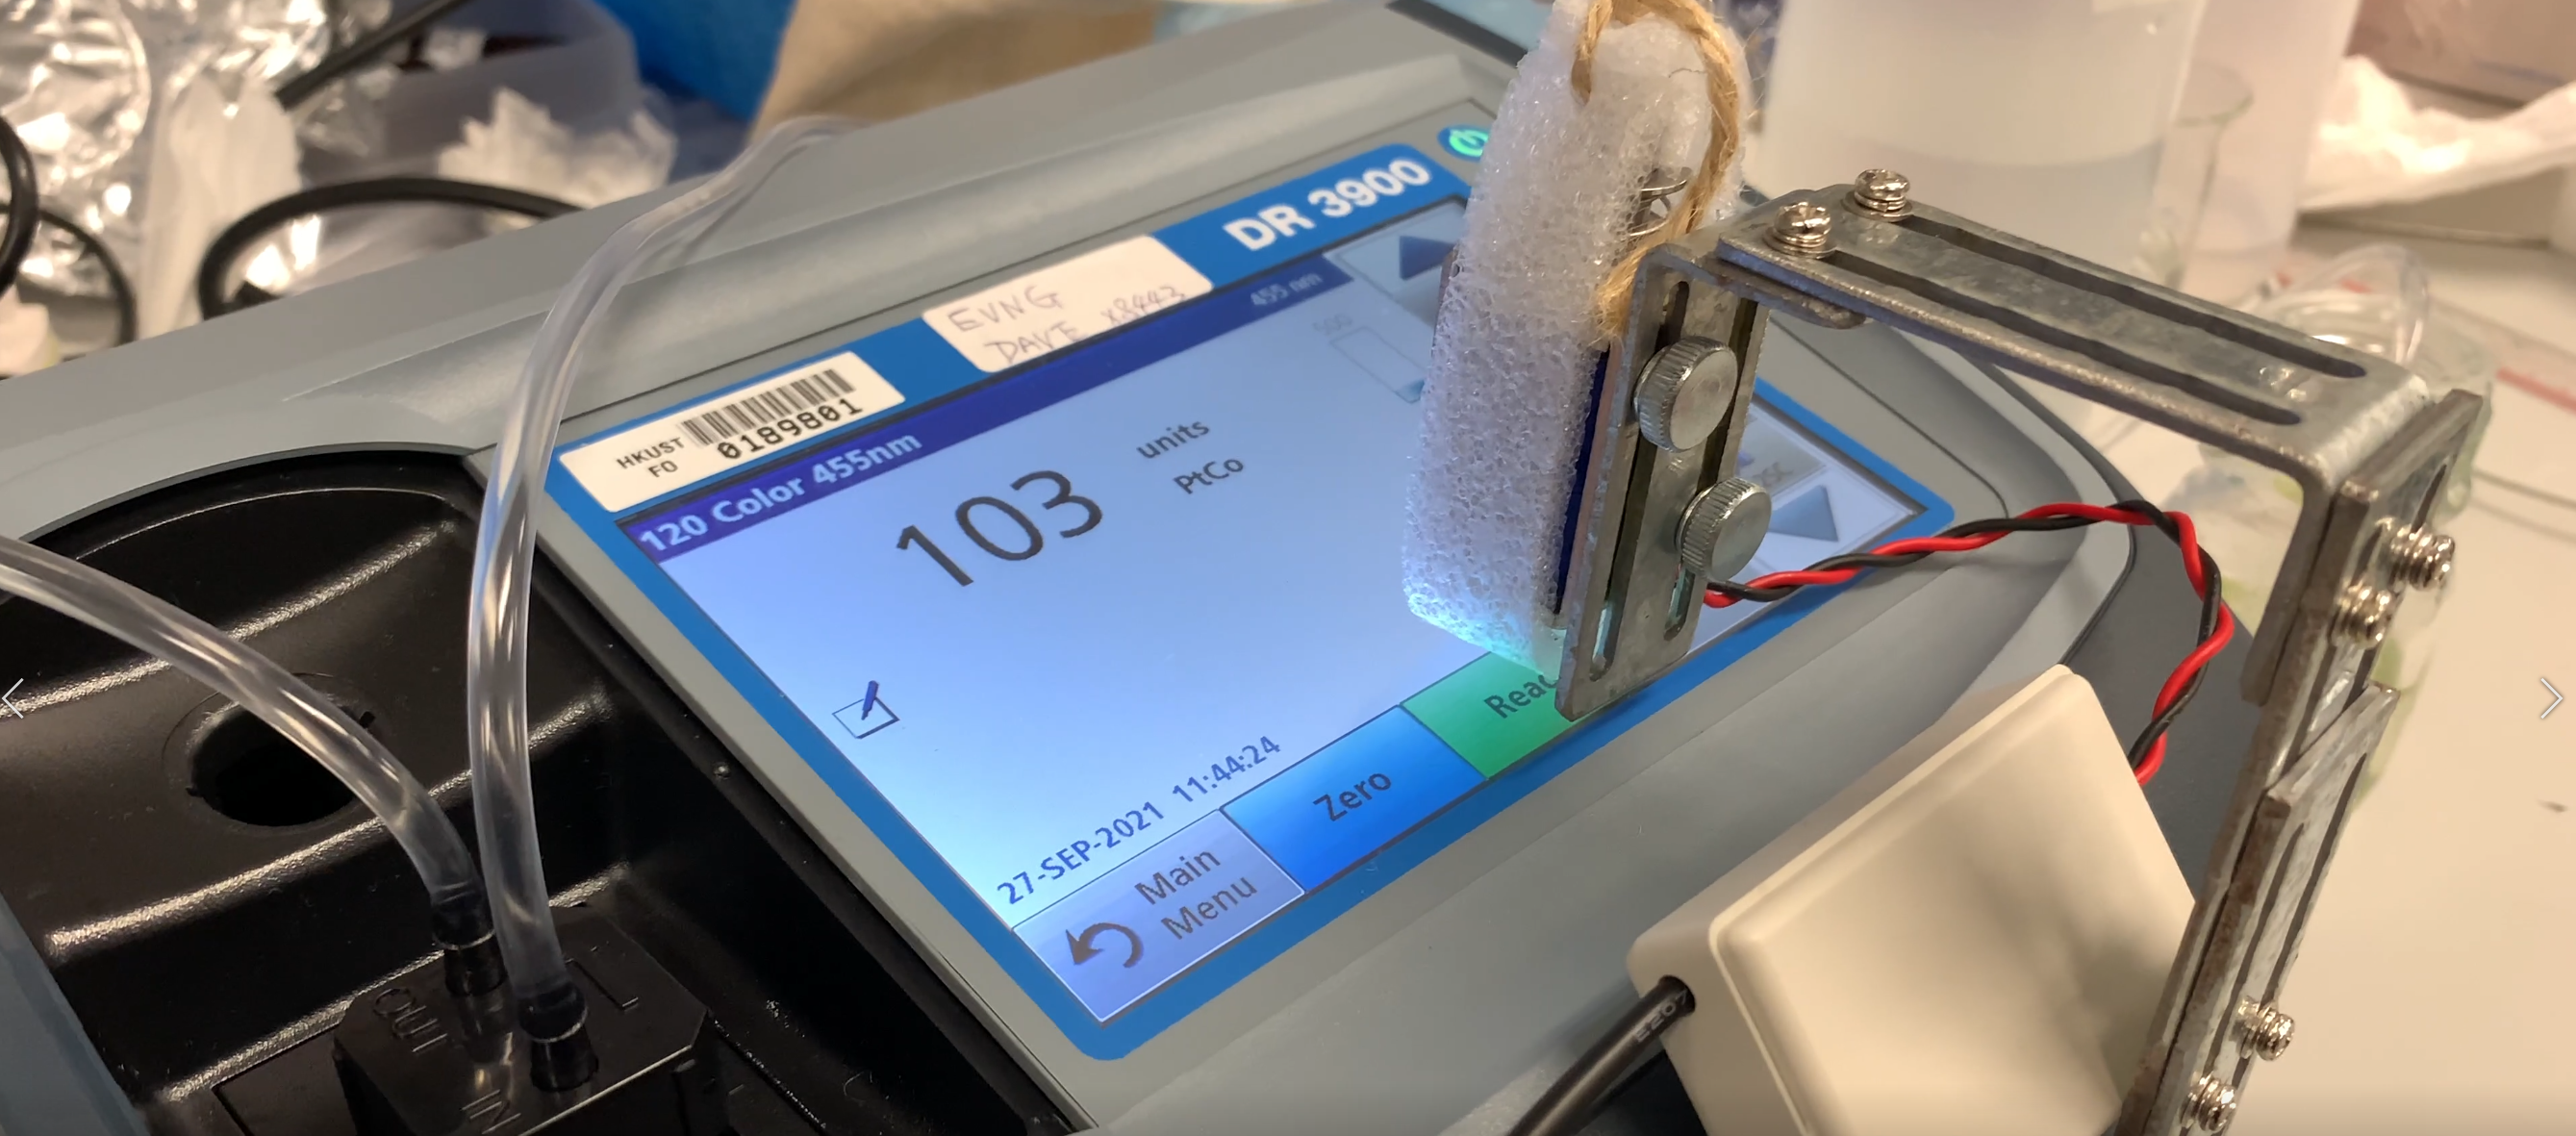
\includegraphics[width=\linewidth]{imgs/instrument/actuator-mount.png}
        \caption{Customized clicker/actuator} \label{fig:hach-actuator}
    \end{subfigure}%  
  \caption{Instruments of on-line colour analysis system.} \label{fig:hach}
\end{figure}

The maintenance and calibration of the DR3900 spectrophotometer is performed on a weekly basis. During the maintenance, the DR3900 device was shut off, and chlorine solution at the concentration of 100 mg/L was pumped into the sampling tubes and the plastic cuvette for disinfection and cleansing. The cleanse of the tubes and cuvette were manually inspected with eyes to make sure no foreign objects were stuck inside. De-ionized water was brought to the site to perform the spectrophotometer calibration after the reboot of DR3900. 

\begin{figure}[h]
    \centering
    \includegraphics[width=0.8\columnwidth]{imgs/instrument/colour-sampler.png}
    \caption{Schematic diagram of the custom-made on-line colour anlaysis system.}
    \label{fig:diagram-colour-analysis}
 \end{figure}

\subsection{Loss function for model evaluation}
Loss functions are used to determine the error between the model outputs (i.e., prediction or forecasting values) and the given target value \citep{deepaiLossFunction2022}. The bigger the difference between the ground truth \boldmath${y}$ and the model outputs \boldmath${\hat{y}}$, the higher the value of the loss function is, meaning the model perfomred poorer. A low value for the loss means the modle perfomred well. The selection of the types of the loss function is essential for training the model to perform specific tasks. In this study, Mean Squared Error (MSE) is used for evaluating the regression models. The values of MSE will never be negative, and is formally defined by the following equation:

\begin{equation}\label{eq-mse}
    MSE=\frac{\sum (y_i-\hat{y_i})^2}{n}
\end{equation}

\subsection{Data cleaning and pre-processing}
The raw data embedded in the original csv files exists many issues, such as missing values, having extreme low or high values, and unreadable texts, etc. Thus, the data cleaning and pre-processing are necessary for more effective process of model training. Python programming language and related modules of Numpy and Pandas were used to clean and pre-process the raw dataset for further usage. The ammonia raw dataset contained 44,640 samples (data points) with 8 variables, giving a matrix size of 44,640 x 8, and the samples were collected in time series at 1 minute interval. The colour level raw dataset contained 1488 samples with 34 variables, giving a matrix size of 1488 x 34, and the samples were collected in time series at 30 minute interval.

Before the high-resolution data from colour and ammonia datasets were compressed into time series data at 1 hour interval via averaging, extreme values were manually removed. For ammonia dataset, we replaced the values higher than 7.0 mg/L with NaN (i.e., Not a number), and futher use interpolation to fill up the NaN along with the missing values in the dataset. For colour dataset, we manually took out the relatively low data points on the days when the maintenance and calibration tasks were performed; extremely values higher than 300 Hazen Unit were also replaced by NaN. Same as the data cleaning method used for ammonia dataset, the missing values and NaN were filled up via interpolation. 

\subsubsection{Data smoothing with Savitzky-Golay and EWMA filter}
Data smoothing was performed on both ammonia and colour datasets using the same method. One of the effective ways to remove the noise from the dataset is to apply data smoothing filters. Two filteres were applied in this study, Savitzky-Golay (SG) and Exponentially Weighted Moving Average (EWMA) filters.

A SG filter is a digital filter that can be applied to a set of digital data points for the purpose of smoothing the data, that is, to increase the precision of the data without distorting the signal tendency. This is achieved, in a process known as convolution, by fitting successive sub-sets of adjacent data points with a low-degree polynomial by the method of linear least squares. \citep{wikipediaSavitzkyGolayFilter2022}

a polynomial curve based on the  and  Extract short-time window 
Determine polynomial degree
Find the smoothed data point (i.e., at center of the window)
Repeat for shifted window (e.g., similar to moving average)

EWMA

\begin{figure}[h]
    \centering
    \begin{subfigure}{0.4\textwidth}
      \includegraphics[width=\linewidth]{imgs/pre-processing/demo-polynomial-fitting.png}
      \caption{SG filter with different polynomial degree \citep{taalSmoothingYourData2017}.} \label{fig:filters-sg}
    \end{subfigure}%
    \hspace{3em}%   % maximize separation between the subfigures
    \begin{subfigure}{0.5\textwidth}
      \includegraphics[width=\linewidth]{imgs/pre-processing/demo-weight-ewma.png}
      \caption{EWMA weight with varied alpha values \citep{cfiExponentiallyWeightedMoving2022}.} \label{fig:filters-ewma}
    \end{subfigure}%  
  \caption{Illustration of the influence of different polynomial degrees in the fitting of SG filter and the weigth decay with varied alpha values in EWMA filter.} \label{fig:filters}
\end{figure}

\subsubsection{Outlier Removal}

\subsection{Data transformation}
Split of Train/valid/test dataset 



Most AI techniques were modeled using experimental data to simulate, predict confirm, and optimize contaminant removal in wastewater treatment processes. Experimental data set were either divided into three parts (training, validation, and testing) or two parts (training and testing). The training set was used to develop the model, the validation data set was used to optimize the model, and the testing data set was used to test the model in the prediction stage.

\section{Architecture design of the selected baseline models}
\subsection{The use of software and machine learning framework}
Python
pytorch
\subsection{Random Forest}
F can be described as an ensemble method in which the final result is obtained by aggregating (through averaging in the case of regression) results from multiple weak learners known as Classification and Regression Trees (CARTs) (Breiman, 2017). Each weak learner (tree) is trained on the bootstrap set, which is obtained by sampling with replacement from the original training set. For trees, the input variables are used to generate nodes. These variables are selected partially and randomly as a subset in every split, then the variable contributing to the smallest sum of impurity of two child nodes at a certain split point is chosen as the split variable. This is done repeatedly until the trees don't need to split anymore. The regression impurity of a particular node is defined by Eqs. (2), (3) and (4), \citep{wangMachineLearningFramework2021}
\subsection{LSTM}
Recently, deep recurrent neural networks (RNN) such as long short-term memory networks (LSTM) have shown breakthrough results over state-of-the-art machinelearning methods in many applications with non-linear temporal data, including robotics, high-energy physics and computational geometry (Goodfellow et al. 2016). These methods can successfully engineer appropriate long-term temporal dependencies and variable length features, significantly lessening the need to pre-process data with respect to traditional machine-learning methods or statistical approaches. It is the ability to capture the long-term dependencies that make LSTM networks particularity fitting for the problem at hand. 

Fig. 1 The general schema of a RNN unit versus a LSTM one (adapted from Olah 2015)

Architecture of the method proposed by Mamandipoor et al. (2020)

\subsection{RNN}

\subsection{GRU}

\section{Implementation of regularization}

\subsection{Scheduler}


\chapter{Results and Discussion}
\section{Baseline performance}
\section{Pre-processing}


\section{Feature engineering}
\section{Architecture desing}

\chapter{Conclusions and Recommendation}
\section{Conclusions}
\subsection{Machine learning models vs deep learning models}
The selection of using which machine learning and deep learning models was not widely discussed to the best of our knowledge in the modelling of wastewater treatment industry. This study has investigated on the model performance of machine learning model of RF, and four other deep learning models of DNN, RNN, GRU and LSTM on forecasting ammonia concentrations and colour levels in reclaimed water system for assisting treatment operation and management. The evidence from this study suggests deep learning models are much capable in learning from the historical data and generate more accurate forecasting results. In both ammonia and colour forecasting models, the test loss values of RF are much higher than the values from the least performanced deep learning model of DNN. Among all the deep learning models, the results indicate LSTM and GRU models have the lowest test loss of 0.0405 and 0.0414, respectively. However, the further research works suggest LSTM models trained with pre-processing methods generate the lowest test loss compared to GRU, making the LSTM model the most promising recurrent neural network model for training forecasting models.

\subsection{Data pre-processing techniques}
Our research also highlighted the importance of how the model performance can be improved from applying data pre-processing and feature engineering techniques. Generally speaking, all the proposed data smoothing and outlier removal methods reduced the test loss values compared to the baseline model performance (i.e., the window sizes of the filters need to be carefully selected), as showin in Fig.~\ref{fig:preprocessing-comparison}. It is believed that the convoluted datapoints generated from data smoothing filters enable the recurrent neural networks to predict the future values more easily.

%This paper has investigated on how much the data pre-processed methods and feature engineering techniques can improve the performance on the ammonia and colour forecasting models. The evidence from this study suggests ammonia forecasting model trained by SG filter (i.e., LSTM-1-sg7) reduced test loss by 4.2\%, and model trained with engineered features (i.e., LSTM-4-sg7) reduced test loss by 8.9\%. Showing 

\subsection{Feature engineering}
This study is the first step towards enhancing our understanding to the potential benefits of using created features for model training. The thorough examinations of the Geomap nearby the SHWEPP and the investigation of water composition in the public sewege system helped us to hypothesize that the change of ammonia concentrations and colour levels are dependent to each other. With the help of additional colour/ammonia data for ammonia/colour forecasting model, the test loss reduced by 6.4\% (i.e., LSTM-2-sg7 compared to LSTM-1-obs) and 10.8\% (i.e., LSTM-2-ew4 compared to LSTM-1-obs), respectively. 

Moreover, the similarity between the household consumption patterns and the daily fluctuation of ammonia concentrations have unexpectedly helped us to formulate the time features via positional encoding. The influence of the sine and cosine hour features on the model perfromance showed tremendous improvements on both ammonia and colour forecasting models. In the former, test loss dropped by 8.9\% (i.e., LSTM-1-obs compared with LSTM-4-sg7) while the latter reduced by 28.6\% (i.e., LSTM-1-obs compared with LSTM-3-sg9). The remarkable use of positional encoding features is it is not limited to just ammonia and colour forecasting models. Any time series data characterized with daily fluctuation patterns can adopt the use of the features of sine and cosine hour as long as the patterns are based on actaul events. In addition, the positional encoding features are not limited to hour, we can encode features into from seconds to weeks, and even years, the application of it is infinite. However, the feature engineering method clearly has some limitations. In the results of ammonia forecasting models, LSTM-2-obs, LSTM-3-obs and LSTM-4-obs showed higher tess loss compared to LSTM-1-obs, indicating when the models were trained by any features other than ammonia, the model performance worsened. In addition to that, when extra features were train with EWMA filters, the test loss increased, and the worsening of model performance also occured on colour forecasting models trained by EWMA filters. Our results suggest that feature engineering needs to be carefully evaluated and experimented before the real use. Despite the limitations, the combination use of feature engineering in building ammonia and colour forecasting models in this study has fully proved it's advantages. 

\section{Recommendations for future research}
Due to the insufficient ammonia and colour data, we cannot differentiate whether the undesired model performance was caused by the heterogeneity of the training and testing datasets or caused by the pre-processing and feature engineering methods we applied on the datasets. It is recommended a larger dataset (e.g., dataset with the size of 2 months or longer) should be used in the future study when evaluating the proposed methods in this study. The insufficient amount of data could also lead to the unstable performance of different models trained by the same data smoothing methods. For instance, LSTM-4-sg7 and LSTM-3-sg7 have the lowest test loss among LSTM-4 and LSTM-3 models, however, LSTM-2-ew4 has the lower test loss than LSTM-4-sg7. We failed to explain what has caused such outcome. 

All the forecasting models in this study only focus on predicting ammonia concentration and colour levles, and in the futher study, more water quality parameters should be included. In reclaimed water system, the concentration of water quality parameters such as turbidity and E. coli are also regulated by Water Supply Department. The violation of any water quality parameter will directly lead to the disqualification of being used as reclaimed water. Moreover, The hidden correlations reside between each water quality parameter will most likely be helpful in building any water quality forecasting models.



% \showthe\font
%%%%%%%%%%%%%%%%%%%%%%%%%%%%%%%%%%%%%%%%%%%%%%%%%%%%%%%%%%%%%%%%%%%%%%%%%
%                                                                       %
%      9) BIBLIOGRAPHY                                                  %
%                                                                       %
% This example uses bibtex to generate the required Bibliography. Refer %
% to the % the file ustthesis_test.bib for the entries of the           %
% Bibliography. Note that only the cited entries are printed.           %
%                                                                       %
% If BibTeX is not used to typeset the bibliography, replace the        %
% following line with the \begin{thebibliography} and \end{bibliography}%
% commands (the "thebibliography" environment) to process the           %
% Bibliography.                                                         %
%                                                                       %
%%%%%%%%%%%%%%%%%%%%%%%%%%%%%%%%%%%%%%%%%%%%%%%%%%%%%%%%%%%%%%%%%%%%%%%%%

%%%%%%%%%%%%%%%%%%%%%%%%%%%%%%%%%%%%%%%%%%%%%%%%%%%%%%%%%%%%%%%%%%%%%%%%%
%                                                                       %
% The recommended bibliography style is the IEEE bibliography style.    %
% "ustbib" defines the IEEE bibliography standard with the added        %
% ability of sorting the items by name of author.                       %
%                                                                       %
% If you are not using BibTeX to process your Bibliography, comment out %
% the following line.                                                   %
%                                                                       %
%%%%%%%%%%%%%%%%%%%%%%%%%%%%%%%%%%%%%%%%%%%%%%%%%%%%%%%%%%%%%%%%%%%%%%%%%

\bibliographystyle{plainnat}

\bibliography{MPhil-thesis-papers}

%%%%%%%%%%%%%%%%%%%%%%%%%%%%%%%%%%%%%%%%%%%%%%%%%%%%%%%%%%%%%%%%%%%%%%%%%
%                                                                       %
%     10) APPENDIX (If Any)                                             %
%                                                                       %
%                                                                       %
%%%%%%%%%%%%%%%%%%%%%%%%%%%%%%%%%%%%%%%%%%%%%%%%%%%%%%%%%%%%%%%%%%%%%%%%%
%\chapter{Python codes}
\section{Python codes for machine learning models}
Random Forest
\begin{lstlisting}    
    model = RandomForestRegressor(n_estimators = 500)
    \end{lstlisting}

Deep Neural Network
\begin{lstlisting}
    class model_MLP_1(torch.nn.Module):
    def __init__(self, n_input=1, n_hidden=10, 
    n_batch=1, n_output=1):
        super(model_MLP_1, self).__init__()
        self.input_size = n_input
        self.hidden_size  = n_hidden
        self.batch_size = n_batch
        self.output_size = n_output
        self.fc1 = nn.Linear(self.input_size, self.hidden_size)
        self.relu = nn.ReLU()
        self.fc2 = nn.Linear(self.hidden_size, self.output_size)
        
    def forward(self, src, device):
        output = self.fc1(src[:,:,0]
        output = self.relu(output)
        output = self.fc2(output)
        return output  
    \end{lstlisting}

Recurrent Neural Network
\begin{lstlisting}
    class RNN(nn.Module):
    def __init__(self, input_size=1, hidden_size=10, 
    num_layers=1, output_size=1):
        super(RNN, self).__init__()
        self.input_size = input_size
        self.hidden_size = hidden_size
        self.num_layers = num_layers
        self.output_size = output_size
        self.rnn = nn.RNN(input_size=input_size,
                          hidden_size=hidden_size,
                          num_layers=num_layers)
        self.fc = nn.Linear(hidden_size, output_size)

    def forward(self, src, device):
        h_t = torch.zeros(self.num_layers,1,self.hidden_size)
        out, _ = self.rnn(src[:,:,0], h_t)
        out = self.fc(out)
        return out   

    \end{lstlisting}

Gated Recurrent Unit
\begin{lstlisting} 
    class GRU(nn.Module):
    def __init__(self, input_size=1, hidden_size=10,
        num_layers=1,output_size=1):
        super(GRU, self).__init__()
        self.input_size = input_size
        self.hidden_size = hidden_size
        self.num_layers = num_layers
        self.output_size = output_size
        self.gru = nn.GRU(input_size=input_size,
                          hidden_size=hidden_size,
                          num_layers=num_layers)
        self.fc = nn.Linear(hidden_size, output_size)

    def forward(self, src, device):
        h_t = torch.zeros(self.num_layers,1,
        self.hidden_size)
        out, _ = self.gru(src[:,:,0],h_t)
        out = self.fc(out)
        return out
    \end{lstlisting}

Long Short-Term Memory
\begin{lstlisting}
    class model_LSTM_1(nn.Module):
    def __init__(self, n_hidden=10):
        super(model_LSTM_1, self).__init__()
        self.n_hidden = n_hidden
        self.n_layers = 1
        self.lstm = nn.LSTM(input_size = 1, 
        hidden_size = self.n_hidden)
        self.linear = nn.Linear(self.n_hidden, 1)

    def forward(self, src, device):
        h_t = torch.zeros(self.n_layers, 1,self.n_hidden)
        c_t = torch.zeros(self.n_layers, 1,self.n_hidden)
        h_t, c_t = self.lstm(src[:,:,0], (h_t,c_t))
        output = self.linear(h_t)
        return output
    \end{lstlisting}



\end{document}
